\subsection{Advanced Configuration and Power Interface (\gls{acpi})}
The \say{ACPI Component Architecture (\gls{acpica})} is an implementation of a group of software components according to the ACPI specification. It is created with the goal of isolating operating system dependencies to a relatively small translation or conversion layer (the OS Services Layer). This makes the bulk of the ACPICA code independent of any individual operating system.so it can used for new operating systems with no source changes within the ACPICA code itself.

Tthe architecture include below component:
\begin{itemize}
  \item \gls{acpica} Subsystem - independent of OS and kernel which serves the primal ACPI services like the AML interpreter and management of namespace.
  \item \gls{acpica} Subsystem - independent of OS and OS Services Layer for every host OS to serve OS support.
  \item The ASL compiler/disassembler for translating the source code from ASL to AML and also disassembling the ASL source code from the binary ACPI tables if exists.
  \item Many ACPI utilities for running the interpreter in level 3 user space taking out the binary ACPI tables residing in the output result of ACPI Dump utility along with translating ACPICA source code to output format of Linux/Unix.
\end{itemize}

Figure \ref{fig:introduction-acpi-component-architecture} portrays the ACPICA subsystem in relation with the device driver(s), host OS, and the ACPI hardware.

\begin{figure}[!htbp]
	\centering
	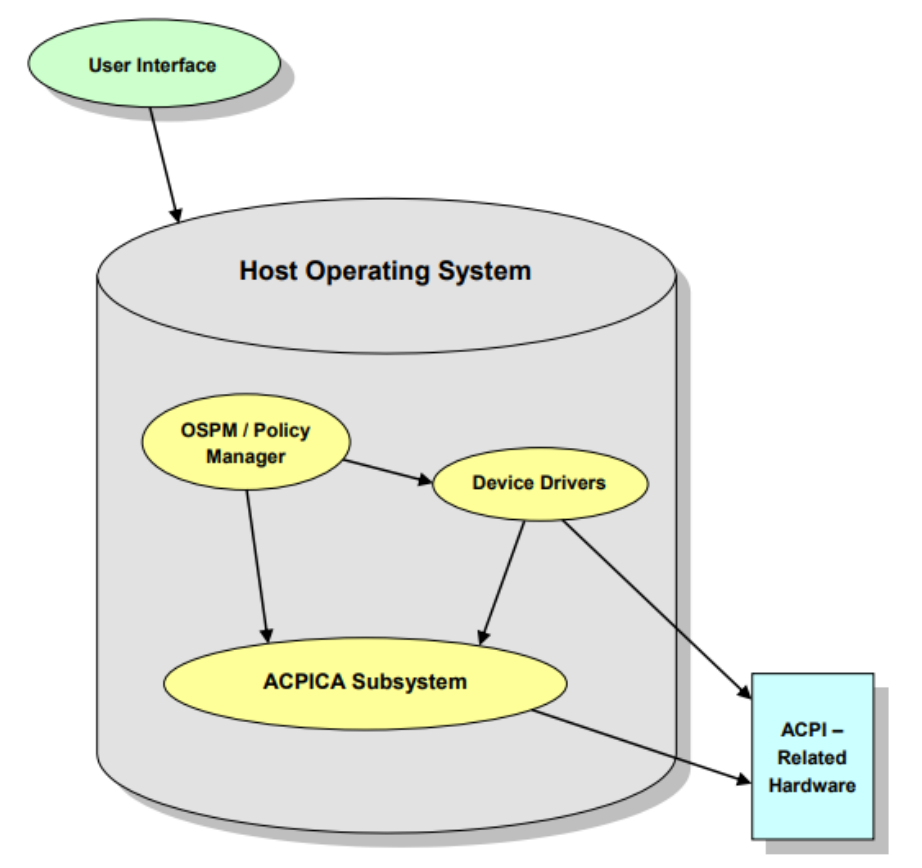
\includegraphics[width=0.8\linewidth]{introduction/acpi-component-architecture}
	\caption{The \gls{acpi} Component Architecture}\label{fig:introduction-acpi-component-architecture}
\end{figure}

\subsubsection{Overview of \gls{acpica} Subsystem}
The \say{\gls{acpica} Subsystem} develops the basic primal aspects of the ACPI specification. Includes an AML parser/interpreter, ACPI table and device support, ACPI namespace management, and event handling. As the ACPICA subsystem serves the lower level services for system, it also involves low-level services of OS like memory management, scheduling, synchronization and I/O.

To allow the ACPICA Subsystem to easily link between any operating system that engage such services, an Operating System Services Layer transforms ACPICA-to-OS requests inside the system calls publicized by the host OS. This OS Services Layer is the one and only element of the ACPICA which pertains source code which is limited to a particular host OS.

%\subsubsection{OS-independent ACPICA Subsystem}
%The OS-independent ACPICA Subsystem supplies the major building blocks or subcomponents that are required for all ACPI implementations — including an AML interpreter, a namespace manager, ACPI event and resource management, and ACPI hardware support.
%
%One of the goals of the ACPICA Subsystem is to provide an abstraction level high enough such
%that the host operating system does not need to understand or know about the very low-level ACPI
%details. For example, all AML code is hidden from the host. Also, the details of the ACPI hardware
%are abstracted to higher-level software interfaces.
%
%The ACPICA Subsystem implementation makes no assumptions about the host operating system or environment. The only way it can request operating system services is via interfaces provided by the OS Services Layer.
%
%The primary user of the services provided by the ACPICA Subsystem are the host OS device drivers and power/thermal management software.
%
\subsubsection{Operating System Services Layer \gls{osl}}
\say{OS Services Layer (OSL)} act as a request translation service for host os from OS-independent ACPICA subsystem. The OSL develops a common subset for interfaces of OS service by utilizing the primitives usable from host OS.

The OSL has to be developed afresh for each and every supported host OS. There exists only one ACPICA Subsystem which OS-independent but there has to be a different OSL for each OS backed by the ACPICA.

The whole ACPICA in relation to the host OS is portrayed in Figure \ref{fig:introduction-acpica-subsystem-architecture}

\begin{figure}[!htbp]
	\centering
	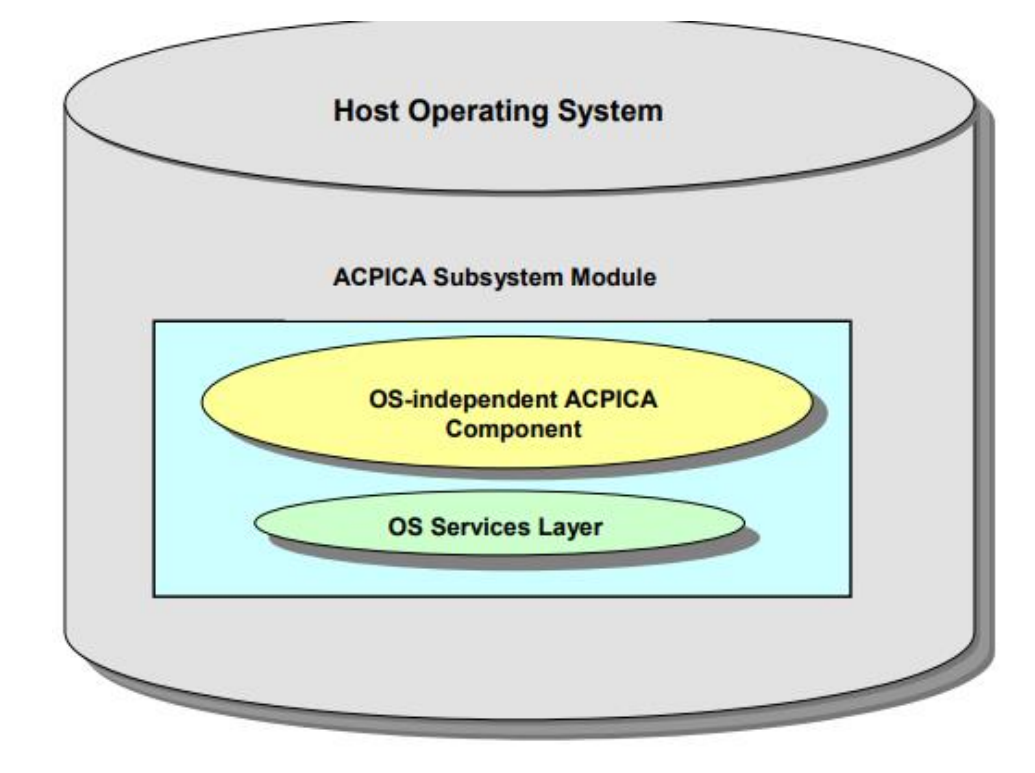
\includegraphics[width=0.7\linewidth]{introduction/acpica-subsystem-architecture}
	\caption{ACPICA Subsystem Architecture}\label{fig:introduction-acpica-subsystem-architecture}
\end{figure}

\subsubsection{\gls{acpica} Subsystem Interaction}
ACPICA Subsystem develops a subset of external interface links that could directly summoned via host OS. These Acpi interfaces serve the literal ACPI services for host. When OS services are needed while servicing of request of an ACPI the Subsystem makes oblique request to host OS through the fixed AcpiOs interfaces. 

\begin{figure}[!htbp]
  \centering
  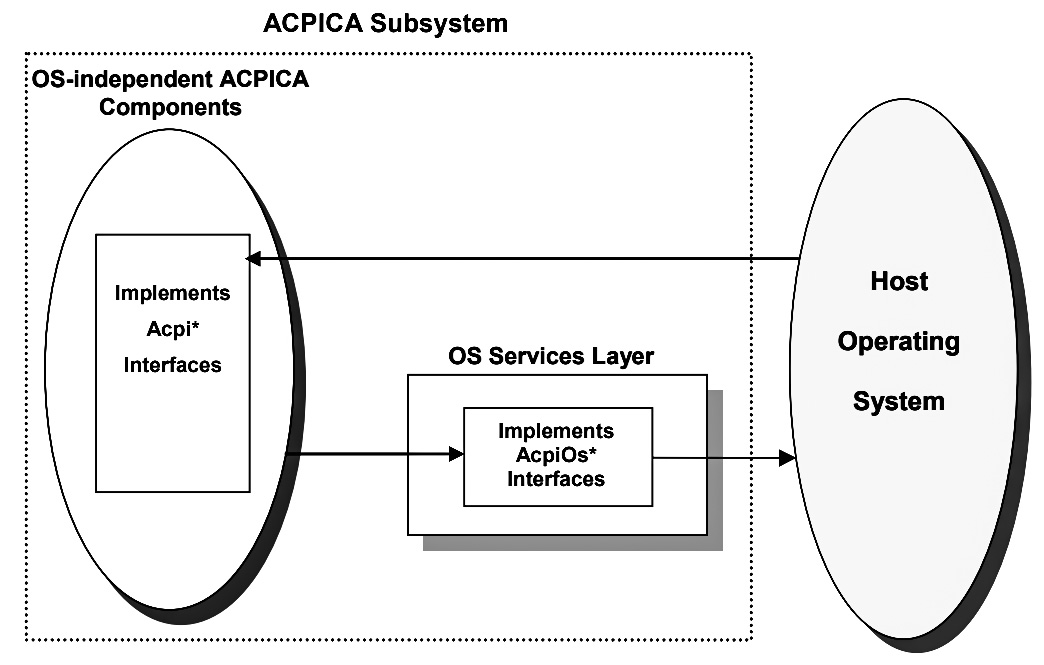
\includegraphics[width=0.7\linewidth]{introduction/acpi-interaction-between-the-architectural-components}
  \caption{Interaction between the Architectural Components}\label{fig:-introduction-acpi-interaction-between-the-architectural-components}
\end{figure}

Figure \ref{fig:-introduction-acpi-interaction-between-the-architectural-components} portrays the kinship and fundamental interaction linking the diverse architectural modules by screening the control flow among them. Note that OS independent ACPICA Subsystem could never call the host OS directly and instead it has to make call(s) to the AcpiOs interfaces inside the OSL. This serves the ACPICA code as OS-independence.
